\documentclass[12pt, oneside]{book}  % jednostranna tlac

%\documentclass[12pt, twoside]{book}  % obojstranna tlac
\usepackage{algorithm}      % For the float environment (optional)
\usepackage{algpseudocode}  % Provides \For, \If, \While, etc.
\usepackage{amssymb}
\usepackage{amsmath}
\usepackage{bm}
\usepackage{multirow}
\usepackage{diagbox}
\usepackage{array}
\usepackage{tabularx}
%spravne nastavenie okrajov
\usepackage[a4paper,top=2.5cm,bottom=2.5cm,left=3.5cm,right=2cm]{geometry}
%zapnutie fontov pre UTF8 kodovanie
\usepackage[utf8]{inputenc}
\usepackage[T1]{fontenc}

%zapnutie slovenskeho delenia slov
%a automatickych nadpisov ako Obsah, Obrázok a pod. v slovencine
%\usepackage[slovak]{babel} % vypnite pre prace v anglictine!

%nastavenie riadkovania podla smernice
\linespread{1.25} % hodnota 1.25 by mala zodpovedat 1.5 riadkovaniu

% balicek na vkladanie zdrojoveho kodu
\usepackage{listings}
% ukazky kodu su cislovane ako Listing 1,2,...
% tu je Listing zmenene na Algorithm 1,2,...
\renewcommand{\lstlistingname}{Algorithm}
% nastavenia balicka listings
% mozete pridat aj language=...
% na nastavenie najcastejsie pouzivaneho prog. jazyka
% takisto sa da zapnut cislovanie riadkov
\lstset{frame=lines}

% balicek na vkladanie obrazkov
\usepackage{graphicx}
% balicek na vkladanie celych pdf dokumentov, tu zadanie
\usepackage{pdfpages}
% balicek na spravne formatovanie URL
\usepackage{url}
% balicek na hyperlinky v ramci dokumentu
% zrusime farebne ramiky okolo liniek aby pdf
% vyzeralo rovnako ako tlacena verzia
\usepackage[hidelinks,breaklinks]{hyperref}


% -------------------
% --- Definicia zakladnych pojmov
% --- Vyplnte podla vasho zadania, rok ma byt rok odovzdania
% -------------------
\def\mfrok{2026}
\def\mfnazov{Analysis of financial markets using machine learning}
\def\mftyp{Bachelor Thesis}
\def\mfautor{Marek Šugár}
\def\mfskolitel{Mgr. Samuel Rosa, PhD. }

\def\mfmiesto{Bratislava, \mfrok}

% študenti BIN a DAV odkomentujú príslušnú dvojicu riadkov
\def\mfodbor{ Computer Science and Mathematics }
\def\program{ Data Science }
% pre BIN:
%\def\mfodbor{ Computer Science and Biology }
%\def\program{ Bioinformatics }
% pre DAV:
%\def\mfodbor{ Computer Science and Mathematics }
%\def\program{ Data Science }

% Uvádzajte pracovisko zo zadania
% u školiteľov z FMFI to bude katedra školiteľa
\def\mfpracovisko{ Department of Applied Mathematics and Statistics  }

\begin{document}   

\frontmatter
\pagestyle{empty}

% -------------------
% --- Obalka ------
% -------------------

\begin{center}
  \sc\large
  Comenius University in Bratislava\\
  Faculty of Mathematics, Physics and Informatics

\vfill

{\LARGE\mfnazov}\\
\mftyp
\end{center}

\vfill

{\sc\large 
\noindent \mfrok\\
\mfautor
}

\cleardoublepage
% --- koniec obalky ----

% -------------------
% --- Titulný list
% -------------------

\noindent

\begin{center}
\sc  
\large
  Comenius University in Bratislava\\
  Faculty of Mathematics, Physics and Informatics

\vfill

{\LARGE\mfnazov}\\
\mftyp
\end{center}

\vfill

\noindent
\begin{tabular}{ll}
Study Programme: & \program \\
Field of Study: & \mfodbor \\
Department: & \mfpracovisko \\
Supervisor: & \mfskolitel \\
% Consultant: & \mfkonzultant \\
\end{tabular}

\vfill


\noindent \mfmiesto\\
\mfautor

\cleardoublepage
% --- Koniec titulnej strany


% -------------------
% --- Zadanie z AIS
% -------------------
% v elektronickej verzii sa zverejňuje zadanie bez podpisov
% v pracach v angličtine anglické aj slovenské zadanie

\newpage
\setcounter{page}{3}

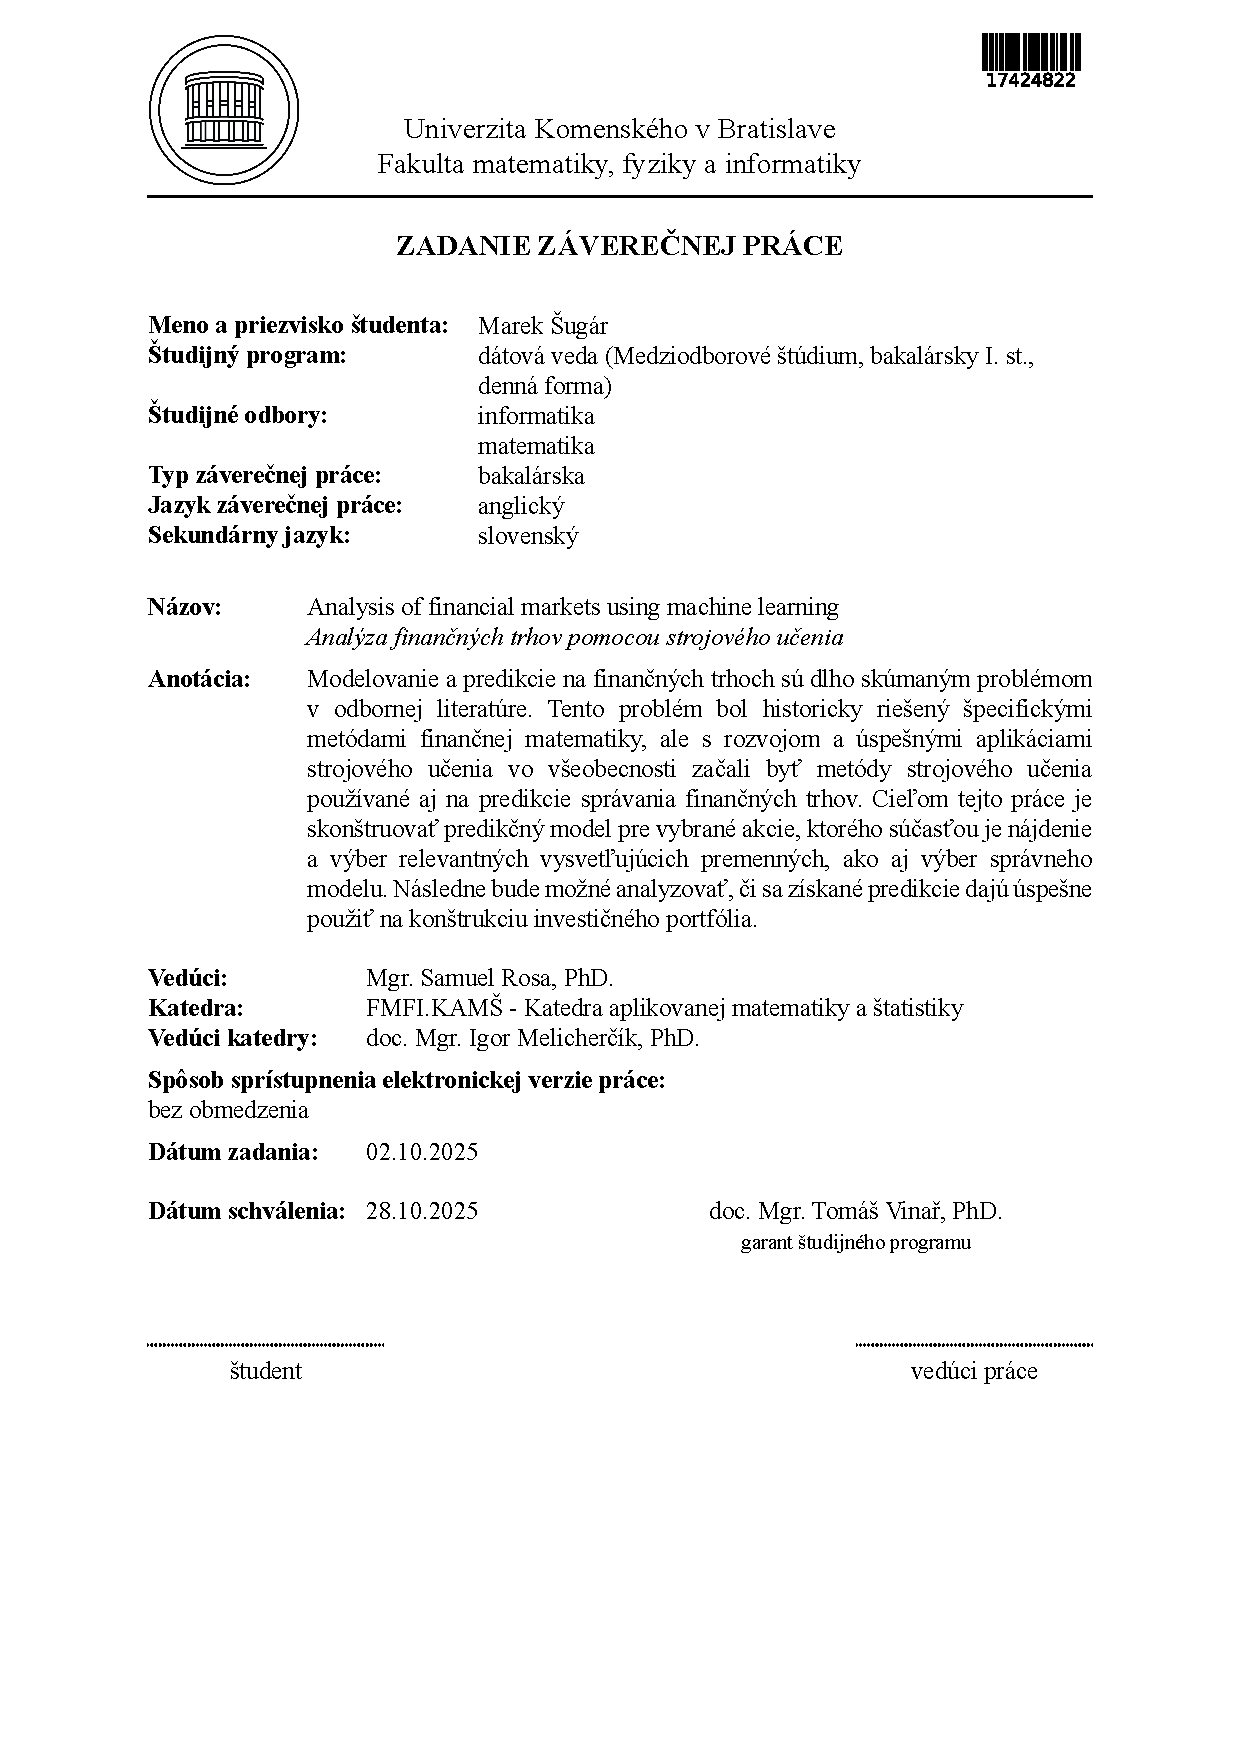
\includepdf{images/zadanieSK.pdf}

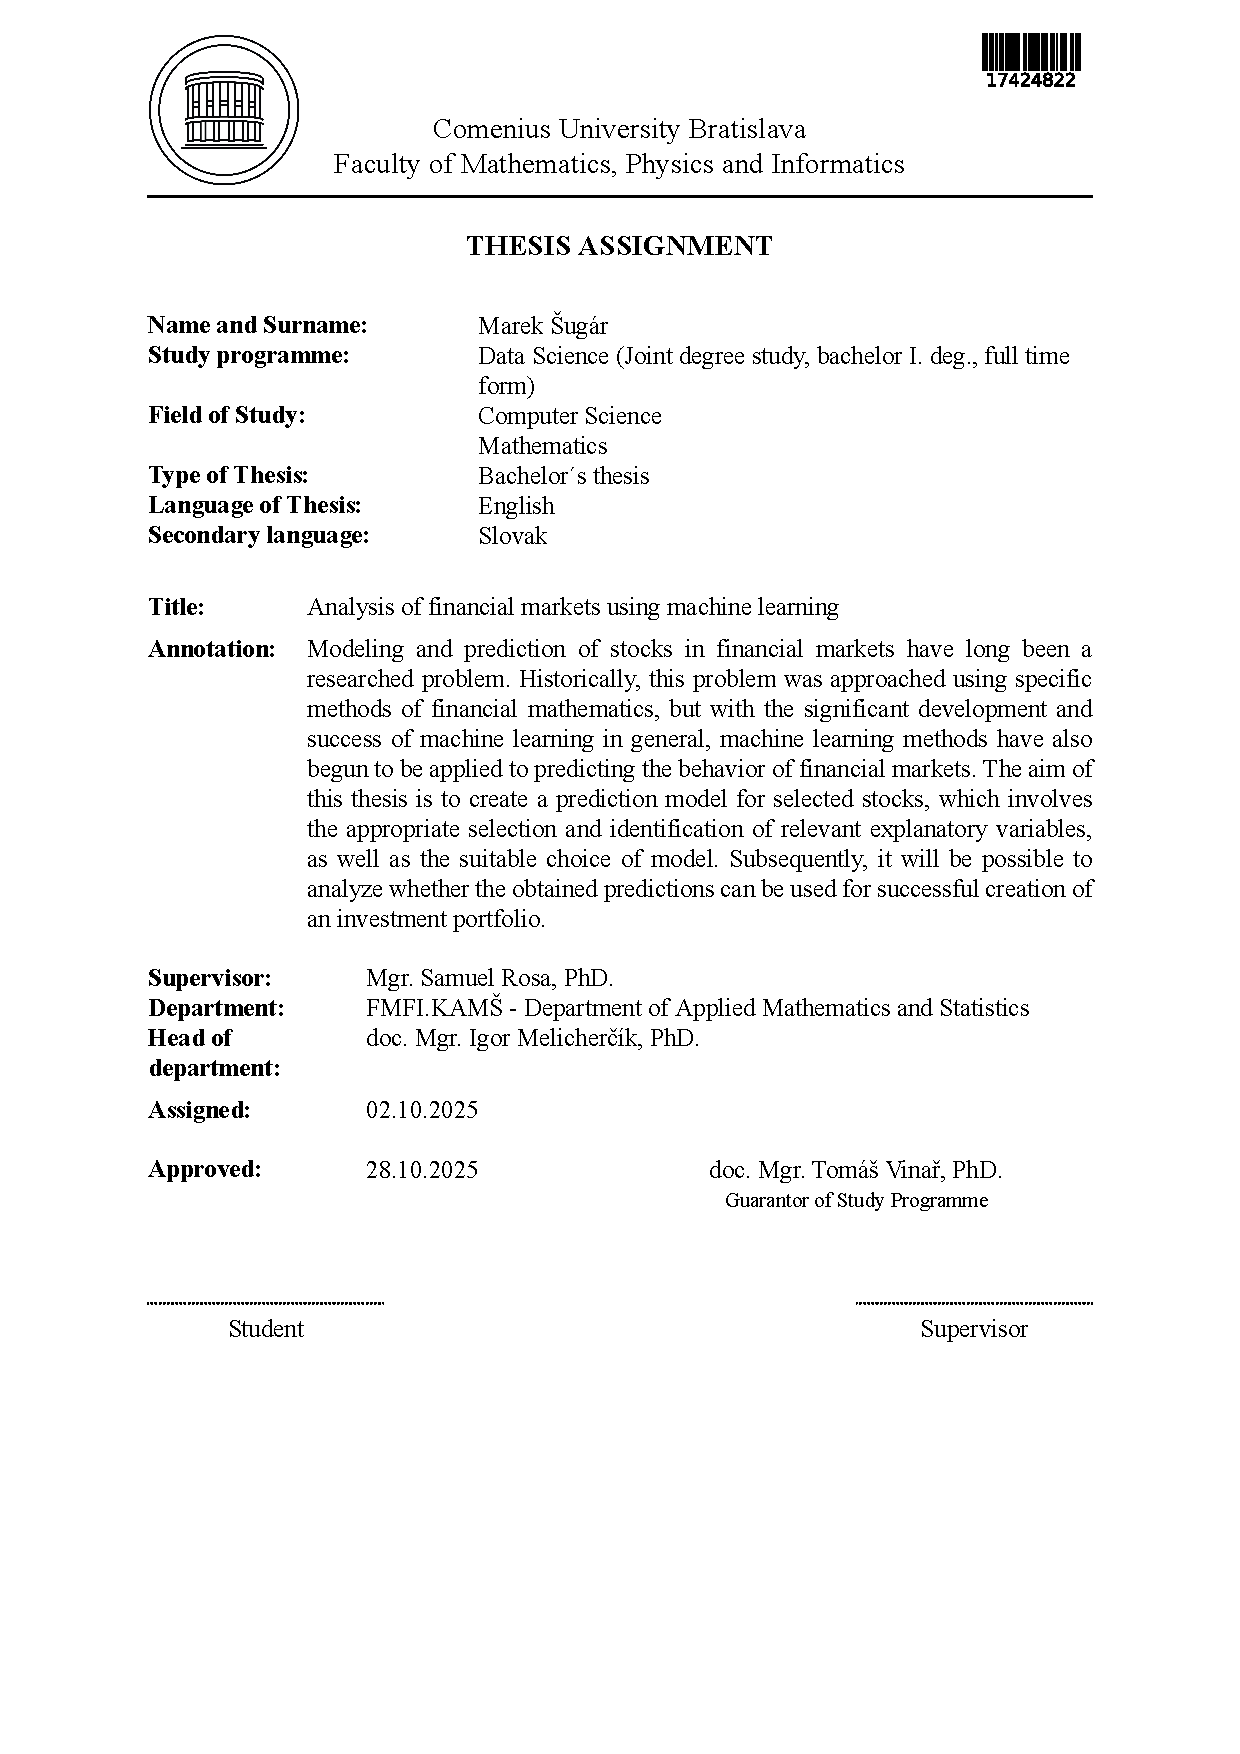
\includepdf{images/zadanieEN.pdf}

% --- Koniec zadania


% -------------------
%   Čestné vyhlásenie a nepovinné poďakovanie
% -------------------
\newpage
\pagestyle{plain}
\paragraph{Declaration:}
I hereby declare that I have independently written this entire
bachelor thesis entitled ``\mfnazov'', including all its
figures and appendices, using the literature listed in the attached
bibliography.

% Uveďte na čo ste nástroje používali
% Podľa typu použitia potom nástroje aj citujte v texte
In preparation of the thesis I have also used the LLM ChatGPT
for the keyword-based searches in particular Python libraries' documentations 
and thesis' grammar checks. I have used artificial intelligence tools in accordance with relevant
legal regulations, academic rights and freedoms, ethical and moral
principles while simultaneously maintaining academic integrity. I am
aware that I am fully responsible for the accuracy of the final text.

\paragraph{Acknowledgments:} This way I would like to thank my supervisor Dr. Rosa, for his mentorship, spent time and intriguing feedback throughout the whole process of thesis' creation.
Last but not least, I would like to express thanks to all my family and friends for their endless support and motivation.

% --- Koniec poďakovania

% -------------------
% --- Abstrakt - Anglicky 
% -------------------
\newpage 
\section*{Abstract}

The goal of the presented bachelor thesis is to evaluate the predictability of the Information Technology (IT) segment of stocks traded on the US stock markets between September 2017 and January 2026. 
Using a unified data-pipeline of selected features, we employ particular regression machine learning (ML) algorithms to predict the next-day closing price of individual stocks.
The used frameworks are Linear regression, Lasso and Ridge regularized regressions, k-Nearest Neighbours, Random Forest Regression, and the ARIMA model. Our results indicate the fairly difficult predictability
of the vast majority of stocks in IT segment. Furthermore, we employ these models in portfolio optimization based on the Markowitz mean-variance portfolio. The study empirically demonstrates that precise predictions have relatively
limited impact on portfolio performance in comparison with market benchmarks.


\paragraph*{Keywords:}  quantitative finance, machine learning, stock markets, predictive analysis

\newpage 
\section*{Abstrakt}

Cieľom predkladanej bakalárskej práce je zhodnotiť prediktabilitu akciového segmentu Informačné Technológie (IT) na akciových burzách v USA v rozmedzí septembra 2017 až januára 2026. Využitím jednotnej sady prediktorov boli
implementované vybrané regresné algoritmy strojového učenia (ML), uspôsobené na predikovanie uzatváracej ceny akcie v nasledujúci deň. Využité algoritmy boli Lineárna regresia, Lasso a Ridge regularizované regresie, k-Nearest Neighbours, Random Forest regresia a ARIMA model.
Výsledky naznačujú relatívnu nízku prediktabilitu značnej väčšiny akcií v IT segmente. Ďalje bol implementovaný algoritmus optimalizácie portfólia na základoch Markowitzovho mean-variance portfólia, ktorý využíva predikcie modelov.
Výsledky práce empiricky demonštrujú relatívne nízky vplyv presných predikcií na výkonnosť portfólia voči trhovým indexom.

\paragraph*{Kľúčové slová:} kvantitatívne financie, strojové učenie, akciové trhy, prediktívna analýza
% --- Koniec Abstrakt - Slovensky

% --- Koniec Abstrakt - Anglicky

% -------------------
% --- Predhovor 
% -------------------
%\newpage 
%
%
%\chapter*{Preface} %
%
%Predhovor je všeobecná informácia o práci, obsahuje hlavnú charakteristiku práce 
%a okolnosti jej vzniku. Autor zdôvodní výber témy, stručne informuje o cieľoch 
%a význame práce, spomenie domáci a zahraničný kontext, komu je práca určená, 
%použité metódy, stav poznania; autor stručne charakterizuje svoj prístup a svoje
%hľadisko. 
%
% --- Koniec Predhovor


% -------------------
% --- Obsah
% -------------------

\cleardoublepage 

\tableofcontents

% ---  Koniec Obsahu

% -------------------
% --- Zoznamy tabuliek, obrázkov, skratiek, slovník - nepovinné
% -------------------

\newpage 

\listoffigures
\listoftables

% ---  Koniec Zoznamov

\mainmatter
\pagestyle{headings}

\input intro.tex 

\input chapter1.tex

\input chapter2.tex

\input chapter3.tex

\input chapter4.tex

\input conclusion.tex



%\input zaver.tex

% -------------------
% --- Bibliografia
% -------------------


\newpage	

\backmatter

\thispagestyle{empty}
\clearpage
\addcontentsline{toc}{chapter}{References}
\bibliographystyle{plain}
\bibliography{literatura} 


% -------------------
%--- Prilohy---
% -------------------

%Nepovinná časť prílohy obsahuje materiály, ktoré neboli zaradené priamo  do textu. Každá príloha sa začína na novej strane.
%Zoznam príloh je súčasťou obsahu.
%
\input appendixA-en.tex

\end{document}
